%%%%%%%%%%%%%%%%%%%%%%%%%%%%%%%%%%%%%%%%%%%%%%%%%%%%%%%%%%%%%%%%%%
%%%%%%%% ICML 2014 EXAMPLE LATEX SUBMISSION FILE %%%%%%%%%%%%%%%%%
%%%%%%%%%%%%%%%%%%%%%%%%%%%%%%%%%%%%%%%%%%%%%%%%%%%%%%%%%%%%%%%%%%

% Use the following line _only_ if you're still using LaTeX 2.09.
%\documentstyle[icml2014,epsf,natbib]{article}
% If you rely on Latex2e packages, like most moden people use this:
\documentclass{article}

% use Times
\usepackage{times}
% For figures
\usepackage{graphicx} % more modern
%\usepackage{epsfig} % less modern
\usepackage{subfigure} 

% For citations
\usepackage{natbib}

% For algorithms
\usepackage{algorithm}
\usepackage{algorithmic}

\usepackage{amsmath}
\usepackage{amssymb}
\usepackage{amsthm}

% As of 2011, we use the hyperref package to produce hyperlinks in the
% resulting PDF.  If this breaks your system, please commend out the
% following usepackage line and replace \usepackage{icml2014} with
% \usepackage[nohyperref]{icml2014} above.
\usepackage{hyperref}

% Packages hyperref and algorithmic misbehave sometimes.  We can fix
% this with the following command.
\newcommand{\theHalgorithm}{\arabic{algorithm}}

\newcommand{\YFcomment}[1]{\marginpar{\footnotesize{{\bf YF:} #1}}}
\newcommand{\SCcomment}[1]{\marginpar{\footnotesize{{\bf SC:} #1}}}

\newtheorem{theorem}{Theorem}
\newtheorem{lemma}[theorem]{Lemma}
\newtheorem{collorary}[theorem]{Collorary}

% Employ the following version of the ``usepackage'' statement for
% submitting the draft version of the paper for review.  This will set
% the note in the first column to ``Under review.  Do not distribute.''
\usepackage{icml2014} 
% Employ this version of the ``usepackage'' statement after the paper has
% been accepted, when creating the final version.  This will set the
% note in the first column to ``Proceedings of the...''
%\usepackage[accepted]{icml2014}


% The \icmltitle you define below is probably too long as a header.
% Therefore, a short form for the running title is supplied here:
\icmltitlerunning{CHANGE ME}

\begin{document} 

\twocolumn[
\icmltitle{TBD}

% It is OKAY to include author information, even for blind
% submissions: the style file will automatically remove it for you
% unless you've provided the [accepted] option to the icml2014
% package.
\icmlauthor{Sunsern Cheamanunkul}{scheaman@eng.ucsd.edu}
\icmladdress{UCSD,
            9500 Gilman Dr., La Jolla, CA 92093}
\icmlauthor{Yoav Freund}{yfreund@eng.ucsd.edu}
\icmladdress{UCSD,
            9500 Gilman Dr., La Jolla, CA 92093}

% You may provide any keywords that you 
% find helpful for describing your paper; these are used to populate 
% the "keywords" metadata in the PDF but will not be shown in the document
\icmlkeywords{boring formatting information, machine learning, ICML}

\vskip 0.3in
]

\begin{abstract} 
TODO
\end{abstract} 

\section{Introduction}
\label{sec:intro}

We consider the $k$-nearest neighbor ($k$-NN) classification rule for
multiclass classification problems where the number of classes $m >
2$. Given a set of training examples, the $k$-NN rule predicts the
label of a new example with the majority of the class labels among its
$k$ nearest neighbors. Fix and Hodges~\cite{Fix1951} show that,
asymptotically, the $k$-NN rule achieves the Bayes error rate by
choosing a large enough $k$ but small compared to the number of
examples $n$. Nonetheless, when $n$ is small, there is no guarantee of
how well the $k$-NN algorithm will perform. 

Additionaly, Cover and Hart~\cite{Cover1967} show that, when $k = 1$,
the aymptotic error rate of the $1$-NN rule is upperbounded by $r^*(2
- \frac{m}{m-1}r^*)$ where $r^*$ denotes the Bayes error rate. This
result suggests that at least a half of the class information is
contained in the nearest neighbor. When the nearest neighbor does not
have all of the class information, it is possible that the missing
class information could be extracted from other examples in the
neighborhood.

In this paper, we propose a modification to the $k$-NN rule which
potentially leverages additional information from the non-majority
class labels in the neighborhood to improve the classification
accuracy. Our approach makes a prediction based on the entire
distribution of the class labels in the neighborhood instead of just
the majority. While the majority rule works well in most cases, it
completely ignores the information from the minority classes which, in
some cases, can contain crucial information.

To motivate our approach, consider the following example. Suppose
there are 3 classes and the examples of each class is generated
according to a normal distribution depicted by
Figure~\ref{fig:toy_example}. Even though the example $x$ in
Figure~\ref{fig:toy_example} is of class A but it is likely that the
majority of class lables in the neighbor of $x$ is class B. In such
case, the majority rule will predict class B. However, if we consider the rest
of the examples in the neighborhood of $x$ and we rarely observe
examples from class C, then a better prediction would have been class A.

\begin{figure}[ht]
\vskip 0.2in
\begin{center}
\centerline{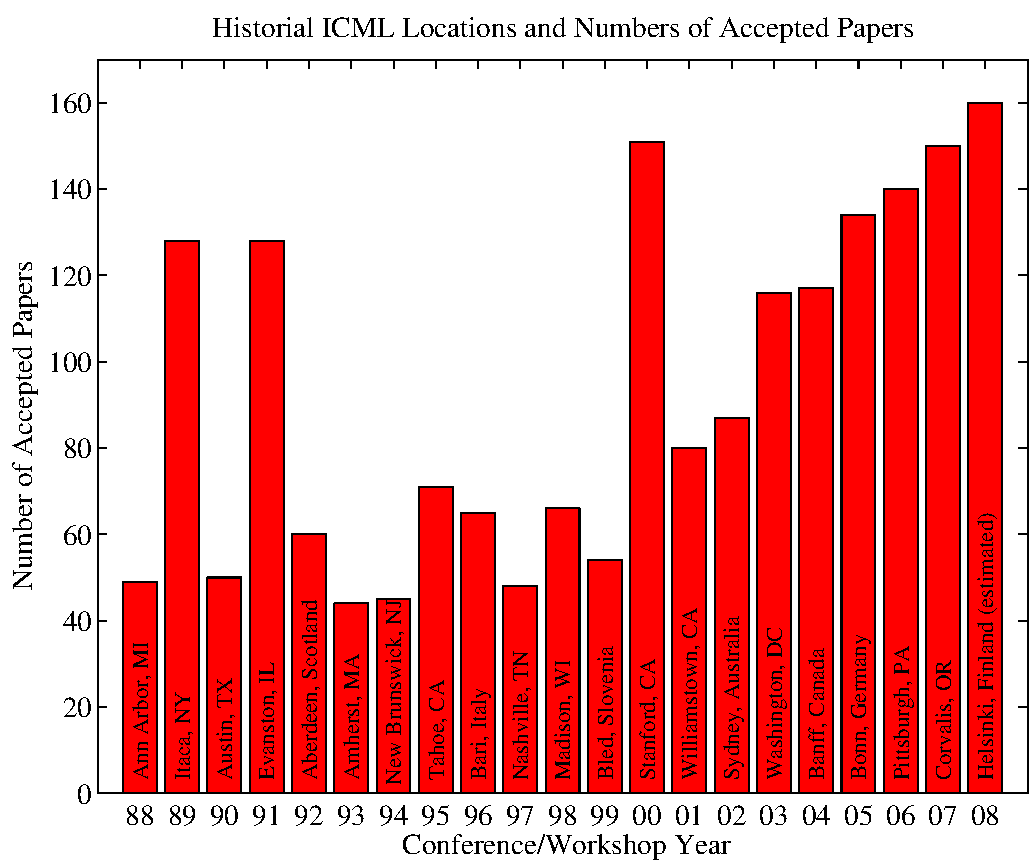
\includegraphics[width=\columnwidth]{icml_numpapers}}
\caption{Toy example}
\label{fig:toy_example}
\end{center}
\vskip -0.2in
\end{figure} 

Our approach can be related to work on learning
label embeddings.~ \cite{Singh-Miller and Collins}, \cite{Dietterich
  Bakiri}, \cite{Allwien, Schapire, Singer}, \cite{Samy Bengio}. The
main difference is that our approach is far more simple , does not
require convex optimization and seemlessly integrated into the $k$-NN
framework. Another related work is \cite{Bilmes} which introduces a
bias term to the likelihood ratio testing that is justified by the
different between the estimated and the true class conditional
probability. 

This paper is organized as follows. In Section~\ref{}, we describe our
approach as well as the analysis of how we justify our algorithm. In
Section~\ref{}, we present experiments comparing our approach with the
traditional $k$-NN algorithm using both synthetic data and real-world
data. Then, we discuss the results in Section~\ref{} and conclude the
paper in Section~\ref{}.

\section{MinKL Approach}

\newcommand{\X}{\mathcal{X}}
\newcommand{\Y}{\mathcal{Y}}
\newcommand{\D}{\mathcal{D}}
\newcommand{\trainset}{\mathcal{S}}
\newcommand{\nh}{\mathcal{N}}

Let $\trainset = \{ (x_1,y_1,) \ldots (x_n,y_n)\}$ be a set of training
examples where each instance $x_i$ belongs to a domain $\X$ with a
metric $d(\cdot,\cdot)$. Without loss of generality, we assume that
each label $y_i$ takes on a value from $\{1,2,\ldots,m\}$. 

Let $\nh_k(x)$ denote the neighborhood of size $k$ of an example $x
\in \X$ with respect to the metric $d$. The traditional $k$-NN
algorithm predicts the label of an example $x$ with the majority of
the labels in $nh_k(x)$. Suppose the true class label $y$ of an
example $(x,y)$ is drawn from a fixed but unknown distribution $p$
whose support is the set of all possible labels. Using the $k$-NN
algorithm, we can estimate $p$ with an empirical distribution $P$
defined by
\[
P(y|x) = \frac{\#\{ \mbox{occurrences of label } y \mbox{ in } \nh_k(x)\}}{k}
\].  It is easy to see that the majority vote rule is equivalent to
the predicting with the maximum likelihood estimate of the true label
assuming the posterior distribution is given by
$P(y|x)$. Specifically, the predicted label $\hat{y}$ is given by
\[
\hat{y} = \arg\max_y P(y|x)
\]

When $n$ is finite, the majority rule can be sub-optimal because the
prediction is made based entirely on the maximum value of the
empirical distribution $P$, which is potentially different from the
true distribution $p$. Sometimes, the class information can be
contained in the non-maximum values of $P$. For example, suppose we
are told that the examples from class A never appears in the
neighborhood of examples from class B and examples from class B and
class C are often confusable. Given a test example $x$, we estimate
$P(B | x) = 0.45$ and $P(C | x) = 0.4$. However, we observe a number
of examples from class A in the neightborhood of $x$. The majority
rule will predict class B disregarding the additional information that
we have and could lead to an incorrect prediction.

\newcommand{\dkl}{D_{\mathrm{KL}}}

To address this problem, we propose a modification to the $k$-NN
algorithm so that it takes into account the entire distribution of $P$
instead of just the maximum coordinate of $P$. We achieve this by
constructing a prototypical distribution for each class. 

\[
Q_i = \int P(y=i|X=x)P(x=X) \vec{P}(y|x=x)
\]

Let $Q_j$
denote the prototypical distribution for class $j$. We can think of
$Q_j$ as a distribution that describes the probability that an example
from class $j$ get confused with other classes. Then, the prediction
is made by minimizing the the distance from $P$ to each of the
prototypical distribution of each class. A simple measure of
difference between any two distributions can be given by the KL
divergence, which is defined as,
\[
\dkl(p || q) = \sum_i p_i \log(\frac{p_i}{q_i})
\]. 

Under certain assumptions, we can show that the class label predicted
by minimizing the KL divergence is the same as the maximum likelihood
estimate (MLE). For any example $(x,y)$, suppose that the class label $y$ is
generated by the following two-step process. First, $j$ is drawn
uniformly from the set $\{1,2,...,m\}$. Then, the class label $y$ is
then drawn from a fixed but unknown distribution $Q_j$. Let $y^k =
[y_1, \ldots, y_k]$ denote a sample of size $k$ drawn IID from an
unknown distribution whose support is the set of all possible
labels. Let $P_{y^k}$ denote a distribution 
induced by the sample $y^k$. Specifically,
\[
P_{y^k}(a) = \frac{\#\{ \mbox{occurrences of } a \mbox{ in } y^k\}}{k}
\]

\begin{lemma}
\label{lemma:1}
For any distribution $Q$ and for any sample $y^k$ (not neccessarily
from $Q$), the likelihood of $y^k$ drawn from $Q$ is given by
\[
P(y^k|Q) = 2^{-k(H(P_{y^k}) + \dkl(P_{y^k} || Q))}
\]
\end{lemma}
\begin{proof}
  \begin{align*}
    P(y^k|Q) 
&= \prod_{i=1}^k Q(x_i)\\ 
&= \prod_{a \in \Y} Q(a)^{nP_{y^k}(a)}\\ 
&= \prod_{a \in \Y} 2^{nP_{y^k}(a) \log Q(a)}\\ 
&= \prod_{a \in \Y} 2^{n(P_{y^k}(a) \log Q(a) - P_{y^k}(a) \log P_{y^k}(a) + P_{y^k}(a) \log P_{y^k}(a))}\\ 
&= 2^{k \sum_{a \in \Y} (-P_{y^k}(a) \log \frac{P_{y^k}(a)}{Q(a)} + P_{y^k}(a) \log P_{y^k}(a) )}\\ 
&= 2^{k(-\dkl(P_{y^k}||Q) - H(P_{y^k}))}\\
  \end{align*}
\end{proof}

\begin{collorary}
\label{col:min_dkl}
Given a set of distributions $\mathcal{Q} = \{Q_1, Q_2, \ldots,
Q_{M}\}$. For any sample $y^k$ drawn from any distribution, $Q_{i^*}
\in \mathcal{Q}$ maximizes the likelihood of $y^k$ among all other
distributions in $\mathcal{Q}$ if and only if $Q_{i^*}$ minimizes the
KL-divergence from $P_{y^k}$.
\[
 i^* = \arg\max_i \log P(y^k|Q_i) = \arg\min_i \dkl(P_{y^k}||Q_i)
\]
\end{collorary}
\begin{proof}
  Applying Lemma~\ref{lemma:1}, we have
  \begin{align*}
    P(y^k|Q_i) &= 2^{-n(H(P_{y^k}) + \dkl(P_{y^k} || Q_i))}\\
    \log P(y^k|Q_i) &= -n(H(P_{y^k}) + \dkl(P_{y^k} || Q_i))\\
    \arg\max_i \log P(y^k|Q_i) &= \arg\max_i - n\dkl(P_{y^k} || Q_i))\\ 
    &= \arg\min_i \dkl(P_{y^k} || Q_i))\\
  \end{align*}
\end{proof}

Next, we justify how to select the prototypical distribution $Q_j$
given a set of training examples $\trainset$. Let $L_k(x)$ denote a sequence
of labels from the neighborhood of size $k$ of the example $x$. A
natural choice is to choose $Q_j$ so that it maximizes the likelihood
of the examples in the training set. More specifically, we want to
solve for $Q_j$ such that, for each label $j \in \{1,2,...,m\}$,
\[
\mbox{maximize } \sum_{(x,y) \in \trainset_j} \log P(L_k(x)|Q_j) \mbox{ subject to } \sum_{i} Q_j(i) = 1 
\]
where $\trainset_j = \{ (x,y) \in \trainset | y = j\}$. We can solve the above program by using Lagrange multipliers,
\[
\nabla_{Q_j(a),\lambda} \left[ \sum_{(x,y) \in \trainset_j} \log P(L_k(x)|Q_j) + \lambda \sum_{i} Q_j(i) \right] = 0
\]
Let $P_x$ denote the empirical distribution over the labels induced by
$L_k(x)$. Using Lemma~\ref{lemma:1}, for each $a$,
\[
\frac{\partial}{\partial Q_j(a)} \sum_{(x,y) \in \trainset_j} \log P(L_k(x)|Q_j) + \lambda
(\sum_{i} Q_j(i)) = \sum_{(x,y) \in \trainset_j} k \frac{P_x(a)}{Q_j(a)} + \lambda = 0
\]
or
\[
Q_j(a) = \frac{k}{\lambda} \sum_{(x,y) \in \trainset_j} P_x(a)
\]
Since $\sum_{i} Q_j(i) = 1$, we have
\begin{align*}
\sum_{a} \frac{k}{\lambda} \sum_{(x,y) \in \trainset_j} P_x(a) &= 1\\
\frac{k}{\lambda} \sum_{a} \sum_{(x,y) \in \trainset_j} P_x(a) &= 1\\
\frac{k}{\lambda} \sum_{(x,y) \in \trainset_j} \sum_{a} P_x(a) &= 1\\
\frac{k}{\lambda} |\trainset_j| &= 1\\
\lambda &= |\trainset_j|k\\
\end{align*}
Plugging $\lambda$ back in,
\[
Q_j(a) = \frac{\sum_{(x,y) \in \trainset_y} P_x(a)}{|\trainset_j|}
\]
In other words, the likelihood is maximized when $Q_j$ is simply the
mean of the posterior estimates over examples from class $j$. The
complete algorithm is given in Algorithm~\ref{alg:minkl}

\begin{algorithm}
\caption{The MinKL $k$-NN algorithm}
\label{alg:minkl}
\begin{algorithmic}[1]
\REQUIRE{A training set $\trainset$ \\ A sequence of the label in
  the neighborhood of size $k$ of $x$, $L_k(x)$. \\ A test example
  $\hat{x}$}
\FOR{$i \in \{1,2,...,m\}$}
\STATE $Q_i \leftarrow [0]^m$
\ENDFOR
\FOR{Each example $(x,y) \in \trainset$}
\STATE {$P_x \leftarrow $ the empirical distribution induced by $L_k(x)$.}
\STATE $Q_y \leftarrow Q_y + P_x$
\ENDFOR
\FOR{$i \in \{1,2,...,m\}$}
\STATE $Q_i \leftarrow Q_i / |\trainset_i|$
\ENDFOR
% \STATE {$P_{\hat{x}} \leftarrow $ the empirical distribution induced by $L_k(\hat{x})$.}
%\STATE $prediction = \arg\min_i \dkl(P_\hat{x} || Q_i)$
\end{algorithmic}
\end{algorithm}

Another potential choice of $Q_j$ is 
\[
Q_j(i) = \delta_j(i)
\]
where $\delta_j(i) = \begin{cases} 1 &\mbox{ if } j = i\\ 0 &\mbox{ otherwise} \end{cases}$.
By using this $Q_j$, for any distribution $P$, the minimizing
KL-divergence decision rule reduces to the majority decision rule.
\begin{align*}
\arg\min_i \dkl(P||Q_i) &= \arg\min_i -\sum_{j} P(j) \log Q_i(j)\\
 &= \arg\max_i P(i)\\
\end{align*}

\section{Experiments}

In this section, we describe experiments we have performed with both
synthetic data and real-world data. Our primary goal is to compare the
classification errors our proposed algorithm (MinKL) with thos of the
traditional $k$-NN algorithm (Majority) under various conditions. 
As for the real-world data, we performed our experiments on two
digit classification datasets: MNIST, SVHN and an online character
recognition dataset: uRight.

\begin{table}[t]
\caption{A summary of the datasets}
\label{table:datasets}
\vskip 0.15in
\begin{center}
\begin{small}
\begin{sc}
\begin{tabular}{lcccr}
\hline
\abovespace\belowspace
Dataset & No. of classes & validation \\
\hline
\abovespace
Synthetic-1   & 10 & 5-fold \\
Synthetic-2 & 81 & 5-fold\\
\belowspace
MNIST & 10 & test set provided\\
SVHN & 10 & test set provided\\
uRight & 26 & 5-fold\\
\hline
\end{tabular}
\end{sc}
\end{small}
\end{center}
\vskip -0.1in
\end{table}

\subsection{Synthetic data}
Our synthetic data can be described as follows. Each instance is a
point in a taurus-like $d$-dimensional hypercube $[0,b-1]^d$. There is
a total of $b^d$ classes and the instances of each class are generated
by a normal distribution with mean located at an integer lattice point
of the hypercube and a covariance matrix $\sigma I_d$. Figure~\ref{}
shows a 2-d representation of each class where $b=5, d= 2$ and $\sigma
= 0.5$. We use Manhattan distance as the similarity measure for the
$k$-NN algorithm.

In the first experiment, we generate a dataset, called Synthetic-1,
using $b=10, d=1$ and $\sigma=1.5$. There is a total of 10 classes in
Synthetic-1. In Figure~\ref{} , we show the 5-fold cross validation
error rate of MinKL and Majority using different $n$ and $k$. Using
the optimal $k$ for each $n$, we compare the error rates of MinKL,
Majority and the Bayes optimal classifier at different $n$ in
Figure~\ref{}. 


Next, we generate a more complex dataset, called Synthetic-2, using
$b=3$, $d=4$ and $\sigma=0.4$. This results in a total of $81$ different
classes. Again, in Figure~\ref{}, we show the 5-fold cross validation
error rate of MinKL and Majority using different $n$ and $k$ and
compare the error rate of MinKL, Majority and Bayes optimal at
different $n$ while $k$ is optimized.


\subsection{MNIST}
Each instance in the MNIST dataset~\cite{} is a 28x28 grayscale image. There
are 60000 training examples and 10000 testing examples. The dataset
has been widely used as a benchmark for classification algorithms. We
prepropress the data by deskewing, resampling the images down to
14x14 pixels, and applying PCA. We transform each image into a feature
vector which is the top 100 PCA components. We use Euclidean distance
as the similarity measure for the $k$-NN algorithm.

The results are summarized in Figure~\ref{}. 

\subsection{SVHN}
The SVHN dataset~\cite{} contains images of digits taken from the Google
street view data. It is considered a harder dataset than the
MNIST. Each instance in the SVHN dataset is a 32x32 RGB image
patch. There are 73257 training examples and 26032 testing
examples. We preprocess the images by deskewing and then extract the
HOG features~\cite{} from the images. We use Manhattan distance as the
similarity measure of the $k$-NN algorithm.

The results are summarized in Figure~\ref{}.

\subsection{uRight}
The uRight dataset is our dataset of handwriting trajectories of
English characters. Each example is a sequence of $(x,y)$-coordinates
representing an English letter. We collected this data from 20
different users writing on a touch screen of a mobile phone. There is
a total of about 10000 examples. The similarity between any two
examples is measured by the dynamic time wraping distance between
them~\cite{}.

We performed the analysis for each user. The 5-fold cross validation
results are shown in Figure~\ref{}.

We also show some of the examples that are misclassified by the
Majority but not the MinKL in Firgure~\ref{}.


\section{Discussion}

From the experiments, we noticed that MinKL approach performs
significantly better than Majority in the small sample situation. As
the number of training examples increases, the gap of the performance
of the two approaches decreases. We anticipated this since the
Majority vote rule is proven to be optimal asymptotically. In some
applications, it is crucial to perform well even when there are only a
few training examples. This is where we believe that our approach has
advantage over the majority vote.

In analysis, we have shown that our approach is optimal when the data
is generated under certain assumptions. For real-world data,
such assumptions may or may not hold. Nonetheless, we can see some
improvements in our experiments. We suspect that our approach will be
more beneficial to problems with a large number of classes and the
confusions between classes are non-uniform. 

In a sense, our approach naturally incoporates the infomation from the
label space into the classification. The label space information is
encoded into the prototypical neighborhood distribution. The
performance of our approach depends on how
different the prototypical neighborhood distributions of different
classes are. If the prototypical distributions are similar, then our
approach will suffer. A workaround is to have multiple prototypical
distributions per class. 

Our approach does not have a consistency gaurantee. It is
possible that our approach will be sub-optimal when the number of
training examples goes to infinity because the prototypical
distribution model is incorrect or insufficent. We do not worry
about this problem that much since we see our approach being used
in a small sample scenario.

In practice, other divergences might work better than the KL
divergence. The KL divergence is considered a special case of a
more general divergence function called Alpha-divergence which is
given by
\[
D^{(\alpha)}_A (p||q) = \frac{1}{\alpha(\alpha - 1)}\left( \sum_1^n
  p^{\alpha}_i q^{1-\alpha}_i - 1\right), \; \alpha \in \mathrm{R} \ \{0,1\}
\]
The KL-divergence can be expressed as $D_{KL} (p || q) = \lim_{\alpha
\rightarrow 1} D^{(\alpha)}_A (p || q)$. 
For uRight dataset, we were able to obtain better classification
accuracy by using Alpha-divergence with $\alpha = 2$.

Our approach can be applied to other classification algorithms as
well. The $k$-NN algorithm is very computational expensive when
classifying a new example. For some applications, it is
important to be able to classify new examples quickly. A simple
modification to the $k$-NN algorithm is to keep a small number of
representatives for each class and discard the rest. This algorithm is
called the $k$ nearest-centroid algorithm ($k$-NC) where only the
$k$-centroids are kept as the class representatives. In the $k$-NC,
the class posterior distribution can be estimating by
\[
p(y|x) = \frac{e^{d(x,C(y))}}{\sum_j e^{d(x, C(j))} }
\]
We can apply the MinKL technique to the class posterior computed this
way. In Figure~\ref{}, we compare the accuracy of the $k$-NC algorithm
with MinKL and Maximum (equavalent to Majority in the $k$-NN).

\section{Conclusions}

We suggest a simple modification to the $k$-NN algorithm.

\bibliography{example_paper}
\bibliographystyle{icml2014}

\end{document} 


% This document was modified from the file originally made available by
% Pat Langley and Andrea Danyluk for ICML-2K. This version was
% created by Lise Getoor and Tobias Scheffer, it was slightly modified  
% from the 2010 version by Thorsten Joachims & Johannes Fuernkranz, 
% slightly modified from the 2009 version by Kiri Wagstaff and 
% Sam Roweis's 2008 version, which is slightly modified from 
% Prasad Tadepalli's 2007 version which is a lightly 
% changed version of the previous year's version by Andrew Moore, 
% which was in turn edited from those of Kristian Kersting and 
% Codrina Lauth. Alex Smola contributed to the algorithmic style files.  
